\chapter{Testy wydajnościowe}
\section{Testy wydajnościowe oprogramowania}
 Testowanie oprogramowanie jest ważnym procesem związanym z jego wytwarzaniem.  Celem testowania jest sprawdzenie czy oprogramowanie jest zgodne ze specyfikacją oraz czy system spełnia oczekiwania klienta. Wykorzystuje się do tego różnego rodzaju testy. Jednymi z nich są testy  sprawdzające wydajność oprogramowania. 

Testy wydajnościowe pozwalają sprawdzić jak oprogramowanie zachowa się w zależności od obciążenia serwera, bazy danych oraz samej aplikacji w oparciu o przygotowane scenariusze użycia oraz wygenerowanych wirtualnych użytkowników, którzy te scenariusze wykonują. Można zbadać, czy nie nastąpi przerwa w działaniu aplikacji, ile czasu będą zajmować poszczególne funkcje aplikacji, jak wykorzystane będą zasoby serwera oraz, czy aplikacja pozwala na skalowanie. Testy wydajnościowe mogą przyjmować różną formę. 

Pierwszą formą są testy obciążeniowe. W takim teście ustala się ilu użytkowników jednocześnie ma korzystać z aplikacji. Na podstawie otrzymanych wyników z takiego testu można zbadać jak aplikacja zachowa się podczas określonego obciążenia oraz otrzymać informacje o czasach odpowiedzi aplikacji.

Drugą formą są testy przeciążeniowe. Pozwalają one określić jak zachowa się aplikacja w warunkach skrajnego obciążenia. Przykładem takiego testu jest zbyt duża liczba użytkowników aplikacji korzystających w tym samym czasie. Dzięki takim testom można zaobserwować między innymi, czy i w jakim momencie aplikacja wyłączy się.

Testy wydajnościowe w aplikacjach internetowych  przeprowadza się, by zbadać jak dużo użytkowników może korzystać z systemu jednocześnie. Takie testy można przeprowadzić zarówno z jednego komputera jak i z kilku. 

W aplikacjach mogą być również badane czasy odpowiedzi aplikacji w zależności od liczby równoległych żądań. Zazwyczaj testy takie są stosowane, gdy aplikacja w swojej specyfikacji ma określony maksymalny czas odpowiedzi przy danej liczbie żądań.

Testy wydajnościowe powinny być prowadzone na środowisku testowym identycznym do produkcyjnego.

\section{Scenariusze testów wydajnościowych wykorzystanych do badań}

Do przeprowadzenia testów wydajnościowych przygotowano dwie aplikacje. Pierwszą z nich była aplikacja w języku \textsl{Java} uruchomiona na dwóch różnych serwerach: \textsl{Tomcat} i \textsl{Jetty}, które obecnie są jednymi z najpopularniejszych rozwiązań służących do uruchamiania aplikacji \textsl{Java}. Drugą była aplikacja w języku \textsl{Go}, która przy użyciu biblioteki \textsl{HttpRouter} \cite{httprouter} pozwala na tworzenie aplikacji działającej jako serwer \textsl{HTTP}.

Każda aplikacja była testowana przez przygotowany zbiór testów w aplikacji \textsl{Apache JMeter}. \textsl{Apache JMeter} pozwala na tworzenie i wykonywanie testów wydajnościowych, symulujących wielu klientów korzystających z aplikacji. Przygotowane testy zostały podzielone na 4 grupy:
\begin{itemize}
    \item testy sprawdzające wydajność walidacji istnienia klucza \textsl{API},
    \item testy sprawdzające wydajność walidacji obiektu \textsl{Cache},
    \item testy sprawdzające wydajność operacji typu \textsl{CRUD},
    \item testy sprawdzające wydajność powyższych scenariuszy równolegle.
\end{itemize}

Pierwsza grupa sprawdza wydajność aplikacji, gdy klient chciał wykonać operacje posiadając nieistniejący klucz \textsl{API}. Na tą grupę składało się pięć testów, wykonywanych w następującej kolejności:
\begin{enumerate}
    \item pobieranie listy wszyskitch obiektów \textsl{Cache},
    \item pobieranie pojedynczego obiektu \textsl{Cache},
    \item tworzenie obiektu \textsl{Cache},
    \item aktualizacja obiektu \textsl{Cache}, 
    \item usunięcie obiektu \textsl{Cache}.
\end{enumerate}
Każde żądanie kończyło się sukcesem, gdy aplikacja zwracała błąd autoryzacji.

Druga grupa testów sprawdza wydajność, gdy klucz \textsl{API} istniał, jednak klient chciał przeprowadzić operacje pobierania, usuwania i aktualizacji nie istniejącego obiektu \textsl{Cache}. Scenariusz grupy wyglądał następująco:
\begin{enumerate}
    \item pobierz nowy klucz \textsl{API},
    \item pobierz obiekt \textsl{Cache} autoryzując się otrzymanym kluczem \textsl{API},
    \item zaktualizuj obiekt \textsl{Cache} autoryzując się otrzymanym kluczem \textsl{API},
    \item usuń obiekt \textsl{Cache} autoryzując się otrzymanym kluczem \textsl{API}.
\end{enumerate}
Każde żądanie kończyło się sukcesem, gdy aplikacja zwracała błąd podczas modyfikacji obiektu \textsl{Cache}.

Kolejną grupą są testy wydajności operacji \textsl{CRUD}. Do przeprowadzenia tej grupy testów został przygotowany zbiór 100 tysięcy losowych wartości w formie pliku \textsl{CSV}. Każda wartość składała się 3 części. Pierwszą był klucz obiektu \textsl{Cache}, natomiast dwie kolejne to wartości, które zostaną zapisane w aplikacji w polu \textsl{value} obiektu. \textsl{Apache JMeter} pozwala na przekazanie pliku \textsl{CSV}, którego wartości można użyć do przeprowadzenia testów. 
Scenariusz tej grupy wyglądał następująco:

\begin{enumerate}
    \item pobierz nowy klucz \textsl{API},
    \item utwórz obiekt \textsl{Cache} o kluczu i wartości otrzymanym z parametru,
    \item pobierz utworzony obiekt \textsl{Cache}, 
    \item zaktualizuj obiekt \textsl{Cache} ustawiając nową wartość pola \textsl{value},
    \item usuń obiekt \textsl{Cache}.
\end{enumerate}
Każdy żądanie oznaczane było jako poprawne, gdy aplikacja nie zwracała błędu.

Ostatnią grupę stanowiły wszystkie testy, opisane w powyższych grupach.

Wszystkie grupy były wykonywane w 15 minutowych cyklach oddzielonych 60 sekundową przerwą.

Każda aplikacja testowana była w czterech przypadkach testowych, które różniły się od siebie liczbą klientów równolegle wykonujących żądania oraz stanem początkowym bazą danych. Były to:
\begin{itemize}
    \item 100 klientów oraz pusta baza danych,
    \item 250 klientów oraz pusta baza danych,
    \item 100 klientów oraz baza danych wypełniona danymi,
    \item 250 klientów oraz baza danych wypełniona danymi.
\end{itemize}
W dwóch ostatnich przypadkach baza danych była wypełniona losowymi danymi: 4000000 obiektów w kolekcji \textsl{api}, 40000000 obiektów w kolekcji \textsl{cache}. Łącznie baza danych zajmowała 12 gigabajtów.

\section{Środowisko testowe}
Do przeprowadzenia testów wydajnościowych wykorzystano 3 serwery wirtualne o poniższych specyfikacjach technicznych: 
\begin{itemize}
    \item 8 rdzeni, 16 gigabajtów pamięci RAM, 160 gigabajtów dysku SSD dla serwera aplikacyjnego,
    \item 4 rdzenie, 8 gigabajtów pamięci RAM, 80 gigabajtów dysku SSD dla serwera bazy danych, 
    \item 4 rdzenie, 8 gigabajtów pamięci RAM, 80 gigabajtów dysku SSD dla serwera, na którym uruchomiony był program \textsl{Apache JMeter}.
\end{itemize}
Serwery komunikowały się po sieci lokalnej (ang. \textsl{LAN}) bezpośrednio między sobą.

Na rysunku \ref{fig:deployment_diagram} zaprezentowany został diagram wdrożenia infrastruktury wykorzystanej do przeprowadzenia testów.
\begin{figure}[!ht]
\centering
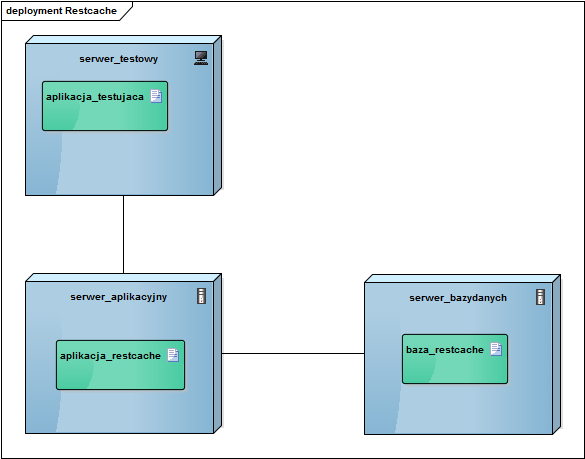
\includegraphics[width=12cm, height=9cm]{\ImgPath/diagram_wdrozenia.png}
\caption{Diagram wdrożenia infrastruktury wykorzystywanej do przeprowadzenia testów}
\label{fig:deployment_diagram}
\end{figure}

